\icode{E-MD-SI-L2-261114-008}
如图所示，斜面体 \(ABC\) 的倾角为\qty{60}{\degree}，\(O\) 点在 \(C\) 点的正上方且与 \(A\) 点等高，现从 \(O\) 点向 \(AC\) 构建光滑轨道 \(OM\)、\(ON\)、\(OP\)，\(M\)、\(N\)、\(P\) 分别为 \(AC\) 的四等分点。一小球从 \(O\) 点由静止开始分别沿 \(OM\)、\(ON\)、\(OP\) 运动到斜面上，所需时间依次为 \(t_M\)、\(t_N\)、\(t_P\)。则\paren[]

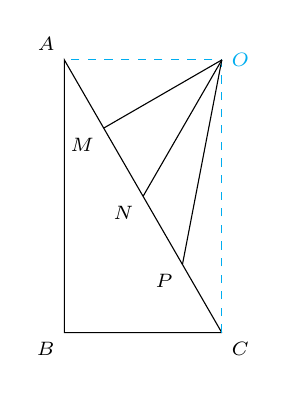
\begin{tikzpicture}[font=\scriptsize]
	\draw (0,0)--(120:4)node[above left]{\(A\)}--(-2,0)node[below left]{\(B\)}--(0,0)node[below right]{\(C\)};
	\draw[dashed,cyan] (0,0)--(0,{2*sqrt(3)})coordinate(o)node[right]{\(O\)}--(120:4);
	\foreach \r/\c in {1/P,2/N,3/M}
		\draw (120:\r)node[below left]{\(\c\)}--(o);
\end{tikzpicture}
\begin{choices}
	\item \(t_M = t_N = t_P\)
	\item \(t_M > t_N > t_P\)
	\item \(t_M > t_P > t_N\)
	\item \(t_M = t_P > t_N\)
\end{choices}
\begin{answer}
    
\end{answer}